%***************************************************
%* Análise e Síntese de Algoritmos
%* Projeto 2 - Abril 2017
%***************************************************
\documentclass[12pt]{article}
\usepackage[utf8]{inputenc}
\usepackage{tikz}
\usepackage{indentfirst}
\usepackage{graphicx}
\usetikzlibrary{arrows.meta}
\renewcommand{\figurename}{Figura}
\renewcommand{\refname}{Referências}
\renewcommand{\familydefault}{\sfdefault}

\usepackage[letterpaper, portrait, margin=3cm]{geometry}

\begin{document}
\title{\vspace{-3cm}Análise e Síntese de Algoritmos}
\author{Grupo 45 - Relatório do Projeto 2}
\date{}

\maketitle

\section*{Introdução}
O presente relatório tem como principal objetivo demonstrar a fundamentação da solução concebida, para o problema proposto.

Este, consiste em construir uma rede de circulação que permita ligar um número finito de cidades entre si, direta ou indiretamente, através de estradas e/ou aeroportos, o mais eficientemente possível, dando prioridade à construção de estradas, sobre a construção de aeroportos.

Dependendo do \textit{input} recebido, há dois \textit{outputs} possíveis:
	\begin{itemize}
		\item Se não for possível construir a rede, é devolvida a mensagem \texttt{Insuficiente};
		\item Caso seja possível construir a rede, são devolvidas duas linhas com as respetivas informações:
		\begin{itemize}
			\item Um único valor correspondente ao custo total de construção da rede;
			\item Dois valores, separados por um espaço em branco, indicando o \textbf{número de aeroportos} e o \textbf{número de estradas} a construir, respetivamente.
		\end{itemize}

	\end{itemize}
Para resolver o problema enunciado, foi desenvolvido um programa na \textbf{linguagem C}.

\section*{Descrição da Solução}
A representação do problema foi feito através de um grafo não dirigido e pesado, cujos vértices correspondem às cidades, e os arcos correspondem às estradas e às ligações entre aeroportos.

\begin{figure}[h]
\centering
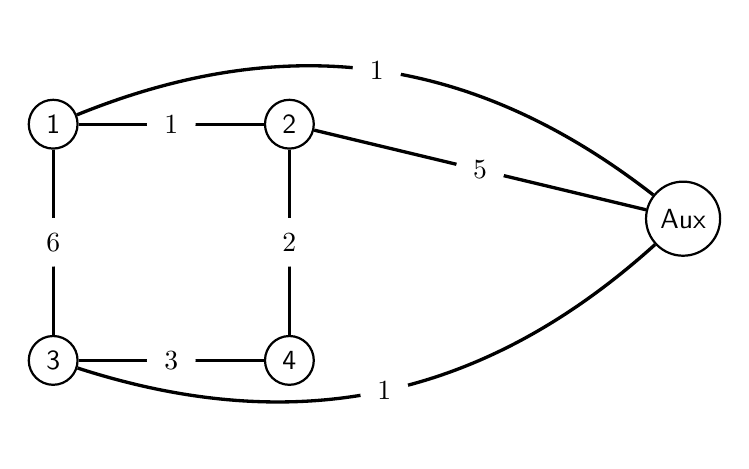
\begin{tikzpicture}


\begin{scope}[every node/.style={circle,thick,draw}]
	\node (4) at (0,0) {4};
	\node (2) at (0,3) {2};
	\node (3) at (-3,0) {3};
	\node (1) at (-3,3) {1};
	\node (0) at (5, 1.8) {Aux};
\end{scope}

\begin{scope}[>={Stealth[black]},
              every node/.style={fill=white,circle},
              every edge/.style={draw=black,very thick}]
	\path [-] (1) edge node {$1$} (2);
	\path [-] (1) edge node {$6$} (3);
	\path [-] (2) edge node {$2$} (4);
	\path [-] (3) edge node {$3$} (4);
	\path [-] (1) edge [bend left] node {$1$} (0);
	\path [-] (2) edge node {$5$} (0);
	\path [-] (3) edge [bend right] node {$1$} (0);

\end{scope}
\end{tikzpicture}
\caption{Representação do \textit{input} 1 do enunciado.}
\end{figure}
Considera-se um vértice auxiliar por forma a representar o custo de construir um aeroporto numa determinada cidade, representado como \textsc{Aux} no exemplo acima. Por exemplo, para se construir um aeroporto na cidade 1 então acrescenta-se um arco de 1 para \textsc{Aux}.

Foi criada uma estrutura de arco (\texttt{edge\_t}) por forma a guardar quais os pares de vértices que o arco liga, assim como o seu peso e tipo (estrada ou aeroporto). Inicializou-se um vetor de estruturas de arco de tamanho $ n_{estradas} + n_{aeroportos} $ por forma a guardar todos os possíveis arcos.

Para a determinação da rede de menor custo, foi aplicado o algoritmo de \textsc{Kruskal}, duas vezes:
\begin{itemize}
	\item Numa primeira vez considerando apenas as estradas;
	\item Numa segunda vez considerando todas as ligações (aeroportos e estradas);
\end{itemize}

Começa-se por inicializar os conjuntos disjuntos, onde cada cidade ficará num conjunto distinto.
Por forma a otimizar a memória utilizada e evitar a cópia de todos os elementos da estrutura, na ordenação dos arcos, em vez de se copiar a estrutura de todos os arcos, é utilizado um vetor auxiliar de inteiros (\texttt{order}). Assim a ordenação é realizada nesse vetor auxiliar, mas comparando o peso de cada arco presente no vetor de estruturas.
Este será ordenado, através de um quicksort, comparando os pesos dos arcos, no vetor de arcos.

De seguida, é efetuada a operação de \textsc{Find-Set} aos dois vértices do arco: se forem iguais, é porque pertencem ao mesmo conjunto, ou seja, as cidades já estão ligadas; se não, unem-se os conjuntos de cada vértice, através da operação \textsc{Union}. Neste último caso, incrementa-se ainda o número de estradas ou o número de aeroportos, dependendo do caso, e soma-se ainda o peso do arco, ao peso total.

Por fim, e como se dá prioridade à construção de estradas, comparam-se os pesos totais das duas aplicações do algoritmo: se o peso total, utilizando apenas estradas, for menor ou igual que o peso total utilizando estradas e aeroportos, é devolvida a rede com apenas estradas; caso contrário, é devolvida a rede com estradas e aeroportos.

Se estiver perante o caso \texttt{Insuficiente}, significa que existe pelo menos uma cidade que não tem quaisquer arcos. Na prática, basta verificar se o grafo é ligado em ambos os casos (só com estradas e com estradas e aeroportos), ou seja, se o número de ligações, só considerando estradas é \texttt{Insuficiente} então verificamos com estradas e aeroportos, se o mesmo acontecer então o resultado é \texttt{Insuficiente}.


\section*{Análise Teórica}
O algoritmo começa por inicializar todos os conjuntos disjuntos, fazendo \textsc{Make-Set} em cada vértice, logo tem complexidade $O(V)$.

De seguida, ordena os arcos por forma a aceder primeiro aos arcos mais leves. Antes de os ordenar, inicia o vetor auxiliar de inteiros ( $O(V)$ ). Para os ordenar, recorre ao \textsc{Quicksort}, cuja complexidade é $O(E\;log\;E)$ no caso médio e $O(E^2)$ no pior caso.

Por fim, realiza duas operações de \textsc{Find-Set}, cuja complexidade é $O(log\;V)$ como é aplicado a todos os arcos fica $O(E\;log\;V)$. Caso não estejam no mesmo conjunto disjunto, realiza a operação \textsc{Union}, de tempo constante, logo tem complexidade $O(1)$.

Assim, e como o \textsc{Kruskal} é aplicado duas vezes, a complexidade do algoritmo, para o caso em que existe solução e para o caso \texttt{Insuficiente}, é $$O(V + E\;log\;E + E\;log\;V) = O(V + E\;log(VE)).$$
Se os arcos forem introduzidos por ordem crescente então a complexidade é
$$O(V + E^2 + E\;log\;V)$$

\section*{Avaliação Experimental}
Os testes tiveram como \textit{input} vários ficheiros gerados, utilizando o gerador de \textit{inputs} fornecido pelo corpo docente. 
A ferramenta utilizada foi o comando \textbf{\textit{time}}, existente na \textit{bash} do GNU/Linux.

Foi utilizado o programa \textbf{\textit{valgrind}} para efetuar as alocações de memória e corrigir eventuais fugas (\textit{memory leaks}). Foi utilizada uma máquina virtual com sistema operativo Xubuntu, 2 GB de memória RAM.

Consideremos que é possível construir um aeroporto em cada cidade e que o número de estradas a construir é o máximo, isto é, $ n_{estradas} = \frac{n_{cidades}(n_{cidades} - 1)}{2}$, de forma a obter a pior situação (em termos de tempo e memória) a que o programa poderá estar sujeito.

\begin{figure}[h]
	\includegraphics{tempo.png}
	\caption{Gráfico da evolução do tempo de execução em função do número de cidades.}
\end{figure}

\newpage

O tempo de execução, para o caso em que existe solução e para o caso \texttt{Insuficiente}, é logarítmico.

\begin{figure}[h]
	\includegraphics{memoria.png}
	\caption{Gráfico da evolução da memória em função do número de cidades.}
\end{figure}

Podemos concluir que a memória é (quase) linear no número de cidades.

De facto, a utilização da memória aproxima-se do tempo de execução.

\begin{thebibliography}{9}

\bibitem{1}Slides disponibilizados na página da cadeira.

\end{thebibliography}

\end{document}